
\chapter{Первая часть}

	\section{Первый раздел}	

    \lipsum[1-1]
    		
	\section{Второй раздел}
		
        Система уравнения Максвелла \cite{ref-item-1}.
		\begin{equation}
			\label{eq:maxwell}
			\begin{cases}
				\curl \vec{H} &= \vec{J}^{s} + \sigma \vec{E} +
				                 \parderf{\epsilon \vec{E}}{t},	 \\
				\curl \vec{E} &= -\parderf{\vec{B}}{t},			 \\ 
				\divergence \vec{B} &= 0,						 \\
				\divergence \epsilon \vec{E} &= \rho,											
			\end{cases}
		\end{equation}
		где $\vec{E}$ и $\vec{H}$ -- напряженности электрического и магнитного полей
		соответственно, $\vec{J}^{s}$ -- вектор плотностей сторонних токов,
		$\vec{B}$ -- индукция магнитного поля, связанная с напряженностью соотношением
		$\vec{B} = \mu \vec{H}$, $\sigma$, $\rho$, $\epsilon$ и $\mu$ -- свойства среды
		(удельная электропроводность, сопротивление, диэлектрическая и магнитная проницаемости).
		Коэффициент магнитной проницаемости $\mu$ вычисляется как $\mu = \hat{\mu} \mu_0$, где
		$\mu_0 = 4 \pi \cdot 10^{-7}$ -- магнитная проницаемость вакуума,
		а $\hat{\mu}$ -- относительная магнитная проницаемость.
	
	\lipsum[1-2] 
	
	На рисунке \ref{img:latex-logo} представлен логотип системы компьютерной вёрстки \LaTeX{}.
	
	\begin{figure}
		\centering
		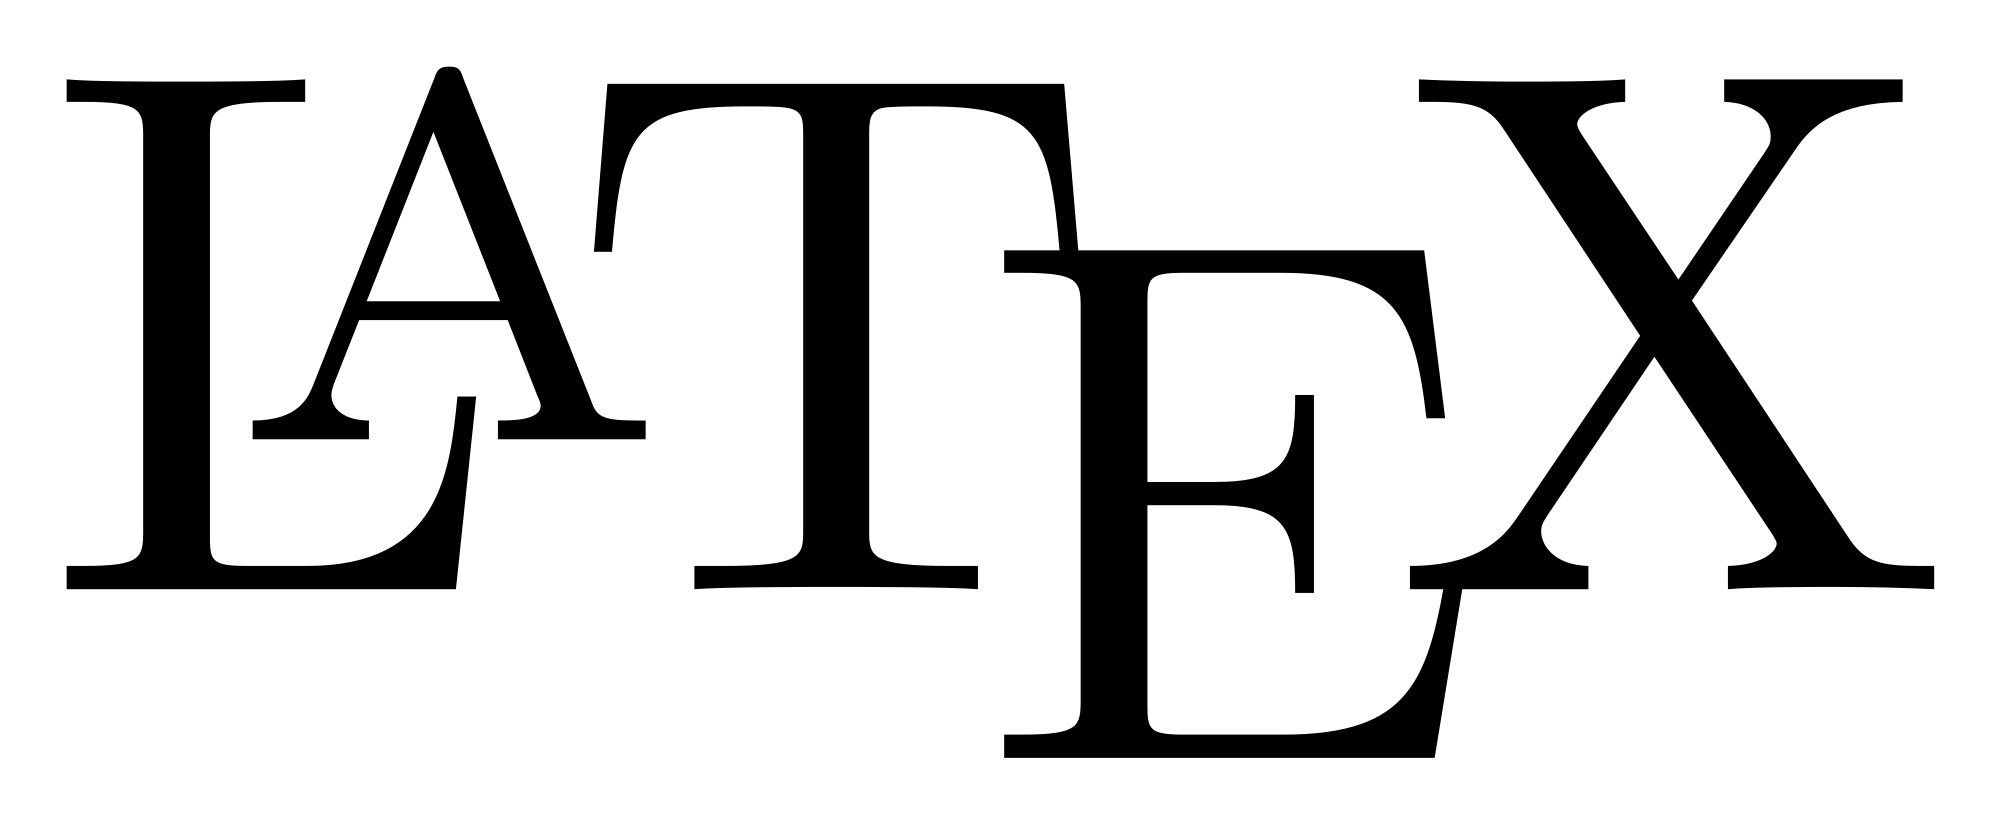
\includegraphics[width=\textwidth]{latex-logo}
		\caption{\LaTeX{} logo}
		\label{img:latex-logo}
	\end{figure}
	
	\lipsum[1]
	
